\documentclass[11pt]{article}

\usepackage{fullpage,fourier,amsmath,amssymb}
\usepackage{listings,color,url,hyperref}
\usepackage{mdframed}
\usepackage{epigraph}
\usepackage[x11names]{xcolor}
\usepackage{gensymb}
\usepackage{forest}
\usepackage{tikz}
\usetikzlibrary{positioning,matrix}

\title{Assignment 5 \\ Sorting: Putting your affairs in order}
\author{Prof. Darrell Long \\ CSE 13S -- Winter 2021}
\date{Due: February 15$^\text{th}$ at 11:59\,pm}

\usepackage{fancyhdr}
\pagestyle{fancy}
\fancyhf{}

\fancypagestyle{plain}{%
  \fancyhf{}
  \renewcommand{\headrulewidth}{0pt}
  \renewcommand{\footrulewidth}{0pt}
  \lfoot{\textcopyright{} 2021 Darrell Long}
  \rfoot{\thepage}
}

\pagestyle{plain}

\definecolor{codegreen}{rgb}{0,0.5,0}
\definecolor{codegray}{rgb}{0.5,0.5,0.5}
\definecolor{codepurple}{rgb}{0.58,0,0.82}

\lstloadlanguages{C,make,python,fortran}

\lstdefinestyle{c99}{
    morekeywords={bool, uint8_t, uint16_t, uint32_t, uint64_t, int8_t, int16_t, int32_t, int64_t},
    commentstyle=\color{codegreen},
    keywordstyle=\color{magenta},
    numberstyle=\tiny\color{codegray},
    identifierstyle=\color{blue},
    stringstyle=\color{codepurple},
    basicstyle=\ttfamily,
    breakatwhitespace=false,
    breaklines=true,
    captionpos=b,
    keepspaces=true,
    numbers=left,
    numbersep=5pt,
    showspaces=false,
    showstringspaces=false,
    showtabs=false,
    tabsize=4
}


\begin{document}\maketitle

\epigraphwidth=0.65\textwidth
\epigraph{\emph{Any inaccuracies in this index may be explained by the
fact that it has been sorted with the help of a computer.}}{---Donald
Knuth, Vol.  III, \emph{Sorting and Searching}}


\section{Introduction}

Putting items into a sorted order is one of the most common tasks in
Computer Science. As a result, there are a myriad of library routines
that will do this task for you, but that does not absolve you of the
obligation of understanding how it is done. In fact it behooves you to
understand the various algorithms in order to make wise choices.

The best execution time that can be accomplished, also referred to as
the \emph{lower bound}, for sorting using \emph{comparisons} is
$\Omega(n \log n)$, where $n$ is the number is elements to be sorted. If
the universe of elements to be sorted is small, then we can do better
using a \emph{Count Sort} or a \emph{Radix Sort} both of which have a
time complexity of $O(n)$. The idea of \emph{Count Sort} is to count the
number of occurrences of each element in an array. For \emph{Radix
Sort}, a digit by digit sort is done by starting from the least
significant digit to the most significant digit. It may also use
\emph{Count Sort} as a subroutine.

What is this $O$ and $\Omega$ stuff? It's how we talk about the
execution time (or space used) by a program. We will discuss it in
class, and you will see it again in your Data Structures and Algorithms
class, now named CSE 101.

The sorting algorithms that you are expected to implement are Bubble
Sort, Shell Sort, Quicksort and Heapsort. The purpose of this
assignment is to get you fully familiarized with each sorting algorithm.
\textcolor{red}{They are well-known sorts. You can use the Python
  pseudocode provided to you as guidelines. Do not get the code for the
sorts from the Internet or you will be referred to for cheating. We will
be running plagiarism checkers.}


\section{Bubble Sort}

\epigraph{\emph{\textbf{C} is peculiar in a lot of ways, but it, like
many other successful things, has a certain unity of approach that stems
from development in a small group.}}{---Dennis Ritchie}

\noindent Bubble Sort works by examining adjacent pairs of items. If the
second item is smaller than the first, swap them. As a result, the
largest element falls to the bottom of the array in a single pass. Since
it is in fact the largest, we do not need to consider it again. So in
the next pass, we only need to consider $n-1$ pairs of items. The first
pass requires $n$ pairs to be examined; the second pass, $n-1$ pairs;
the third pass $n-2$ pairs, and so forth. If you can pass over the
entire array and no pairs are out of order, then the array is sorted.

\medskip
\begin{prelab}{Pre-lab Part 1}
  \begin{enumerate}
    \item How many rounds of swapping do you think you will need to sort
      the numbers ${8, 22, 7, 9, 31, 5, 13}$ in ascending order using
      Bubble Sort?
    \item How many comparisons can we expect to see in the worse case
      scenario for Bubble Sort? Hint: make a list of numbers and attempt
      to sort them using Bubble Sort.
    \item How would you revise the algorithm so the smallest element
      floats to the top instead?
  \end{enumerate}
\end{prelab}

In 1784, when Carl Friedrich Gau{\ss} was only 7 years old, he was
reported to have amazed his elementary school teacher by how quickly he
summed up the integers from $1$ to $100$. The precocious little
Gau{\ss} produced the correct answer immediately after he quickly
observed that the sum was actually 50 pairs of numbers, with each pair
summing to 101 totaling to 5,050. We can then see that:

\[
  n+(n-1)+(n-2) + \ldots + 1 = \frac{n(n+1)}{2}
\]

\noindent so the \emph{worst case} time complexity is $O(n^2)$. However, it could
be much better if the list is already sorted. If you haven't seen the
inductive proof for this yet, you will in the applied discrete
mathematics class.

\begin{pythonlisting}{Bubble Sort in Python}
def bubble_sort(arr):
    n = len(arr)
    swapped = True
    while swapped:
        swapped = False
        for i in range(1, n):
            if arr[i] < arr[i - 1]:
                arr[i], arr[i - 1] = arr[i - 1], arr[i]
                swapped = True
        n -= 1
\end{pythonlisting}


\section{Shell Sort}

\epigraph{\emph{There are two ways of constructing a software design.
    One way is to make it so simple that there are obviously no
    deficiencies, and the other way is to make it so complicated that
    there are no obvious deficiencies. The first method is far more
difficult.}}{---C.A.R. Hoare}

\noindent
Donald L. Shell (March 1, 1924--November 2, 2015) was an American
computer scientist who designed the Shell sort sorting algorithm.
He acquired his Ph.D. in Mathematics from the University of Cincinnati
in 1959, and published the shell sort algorithm in the Communications
of the ACM in July that same year.

Shell Sort is a variation of insertion sort, which sorts pairs of
elements which are far apart from each other. The \emph{gap} between the
compared items being sorted is continuously reduced. Shell Sort starts
with distant elements and moves out-of-place elements into position
faster than a simple nearest neighbor exchange. What is the expected
time complexity of Shell Sort? It depends upon the gap sequence.

The following is the pseudocode for Shell Sort. The gap sequence is
represented by the array \texttt{gaps}. You will be given a gap
sequence, the Pratt sequence ($2^p 3^q$ also called $3$-smooth), in the header file \texttt{gaps.h}.
For each \texttt{gap} in the gap sequence, the function compares all the
pairs in \texttt{arr} that are \texttt{gap} indices away from each
other. Pairs are swapped if they are in the wrong order.

\begin{pythonlisting}{Shell Sort in Python}
def shell_sort(arr):
    for gap in gaps:
        for i in range(gap, len(arr)):
            j = i
            temp = arr[i]
            while j >= gap and temp < arr[j - gap]:
                arr[j], arr[j - gap] = arr[j - gap], arr[j]
                j -= gap
            arr[j] = temp
\end{pythonlisting}

\medskip
\begin{prelab}{Pre-lab Part 2}
  \begin{enumerate}
    \item The worst time complexity for Shell Sort depends on the
      sequence of gaps. Investigate why this is the case. How can you
      improve the time complexity of this sort by changing the gap size?
      Cite any sources you used.
  \end{enumerate}
\end{prelab}


\section{Quicksort}

\epigraph{\emph{If debugging is the process of removing software bugs,
then programming must be the process of putting them in.}}{---Edsger
Dijkstra}

\noindent
Quicksort (sometimes called partition-exchange sort) is, on average, the most
efficient
sorting algorithm. It was Developed by British computer scientist C.A.R. ``Tony''
Hoare in 1959 and published in 1961. It is perhaps the most commonly used
algorithm for sorting (by competent programmers).  When implemented well, it is the fastest
known algorithm that sorts using \emph{comparisons}. It is
usually two or three times faster than its main competitors, Merge
Sort and Heapsort. It does, though, have a worst case performance
of $O(n^2)$ while its competitors are strictly $O(n \log n)$ in
their worst case.

Quicksort is a divide-and-conquer algorithm. It partitions
arrays into two sub-arrays by selecting an element from the array and
designating it as a pivot. Elements in the array that are less than the
pivot go to the left sub-array, and elements in the array that are
greater than or equal to the pivot go to the right sub-array.

Note that Quicksort is an \emph{in-place} algorithm, meaning it doesn't
allocate additional memory for sub-arrays to hold partitioned elements.
Instead, Quicksort utilizes a subroutine called \texttt{partition()}
that places elements less than the pivot into the left side of the array
and elements greater than or equal to the pivot into the right side and
returns the index that indicates the division between the partitioned
parts of the array. In a recursive implementation, Quicksort is then run
recursively on the partitioned parts of the array, thereby sorting each
array partition containing at least one element. Instead of a recursive
Quicksort, you will be writing an \emph{iterative} Quicksort that
utilizes a \emph{stack}. Indices are pushed into the stack two at a
time. The first and second indices represent the leftmost and rightmost
indices of the array partition to sort. Hint: the return type of
partition should be \texttt{int64\_t}.

\begin{pythonlisting}{Partition in Python}
def partition(arr, lo, hi):
    pivot = arr[lo + ((hi - lo) // 2)]; # Prevent overflow.
    i = lo - 1
    j = hi + 1

    while i < j:
        i += 1 # You may want to use a do-while loop.
        while arr[i] < pivot:
            i += 1

        j -= 1
        while arr[j] > pivot:
            j -= 1

        if i < j:
            arr[i], arr[j] = arr[j], arr[i]

    return j
\end{pythonlisting}

\begin{pythonlisting}{Quicksort in Python}
def quick_sort(arr):
    left = 0
    right = len(arr) - 1

    stack = []
    stack.append(left) # Pushes to the end of the stack.
    stack.append(right)

    while len(stack) != 0:
        hi = stack.pop() # Pops off the end of the stack.
        lo = stack.pop()
        p = partition(arr, lo, hi)
        if p + 1 < hi:
            stack.append(p + 1)
            stack.append(hi)
        if lo < p:
            stack.append(lo)
            stack.append(p)
\end{pythonlisting}

\medskip
\begin{prelab}{Pre-lab Part 3}
  \begin{enumerate}
    \item Quicksort, with a worse case time complexity of
      $\operatorname{O}(n^2)$, doesn't seem to live up to its name.
      Investigate and explain why Quicksort isn't doomed by its worst
      case scenario. Make sure to cite any sources you use.
  \end{enumerate}
\end{prelab}

\subsection{Stacks}

You will need to implement the \emph{stack} ADT for your iterative
Quicksort. The following subsections define the interface for a stack.
The header file containing the interface will be given to you as
\texttt{stack.h}. \textcolor{red}{You may not modify this file.} If you
borrow code from any place --- including Prof. Long --- you must cite
it. It is \emph{far better} if you write it yourself.

\subsubsection{\texttt{Stack}}

The stack \texttt{struct} must be defined as follows:

\begin{codelisting}{}
struct Stack {
  uint32_t top;       // Points to the next empty slot.
  uint32_t capacity;  // Number of items that can be pushed.
  int64_t *items;     // Holds the items.
};
\end{codelisting}

This \texttt{struct} \emph{must} be placed in \texttt{stack.c}. The
field \texttt{top} indicates the index that the next pushed item
should go. The field \texttt{capacity} indicates the number of items
that the stack can hold. Finally, the field \texttt{items} is the
underlying array in which items are stored in. The type of each item
will be a \texttt{int64\_t}.

\subsubsection{\texttt{Stack *stack\_create(void)}}

The constructor function for a stack. The \texttt{top} of a stack should
be initialized to 0. The default starting capacity of a stack should be
\texttt{MIN\_CAPACITY}, a macro that is defined in \texttt{stack.h}. The
starting capacity also indicates the amount of memory to allocate for
\texttt{items}.

\subsubsection{\texttt{void stack\_delete(Stack **s)}}

The destructor function for a stack. Remember: your program \emph{must}
be free of memory leaks.

\subsubsection{\texttt{bool stack\_empty(Stack *s)}}

This functions checks if the specified stack is empty or not. If the
stack is empty, return \texttt{true}. Otherwise, return \texttt{false}.

\subsubsection{\texttt{bool stack\_push(Stack *s, int64\_t x)}}

You may notice that the interface does not include a function to check
if a specified stack is full or not. This is because you will be
implementing a \emph{dynamically} growing stack, as demonstrated in
lecture. If the \texttt{top} of the stack matches its \texttt{capacity},
double the capacity and use \texttt{realloc()} to reallocate the memory
that \texttt{items} points to. The amount of memory to reallocate is
given by the new capacity. In the event that reallocating this memory
fails, return \texttt{false}. Otherwise, push item \texttt{x} into the
stack and return \texttt{true} to indicate success.

\subsubsection{\texttt{bool stack\_pop(Stack *s, int64\_t *x)}}

Pops an item off the specified stack, passing the value of the item back
through the pointer to \texttt{x}. Hint: you will need to dereference
\texttt{x} in order to change the value in the memory \texttt{x} is
pointing to. If the specified stack is empty prior to popping, return
\texttt{false}; you cannot pop an empty stack. Otherwise, pop an item
off the stack, pass it back using \texttt{x}, and return \texttt{true}
to indicate success.

\subsubsection{\texttt{void stack\_print(Stack *s)}}

This is a debug function that you should write early on. It will help
greatly in determining whether or not your stack implementation is
working correctly.


\section{Heapsort}

\epigraph{\emph{Increasingly, people seem to misinterpret complexity as
sophistication, which is baffling -- the incomprehensible should cause
suspicion rather than admiration.}}{---Niklaus Wirth}

Heapsort, along with the heap data structure, was invented in 1964 by
J. W. J. Williams. The heap data structure is typically implemented as a
specialized binary tree. There are two kinds of heaps: \emph{max} heaps
and \emph{min} heaps. In a max heap, any parent node \emph{must} have a
value that is greater than or equal to the values of its children. For a
min heap, any parent node \emph{must} have a value that is less than or
equal to the values of its children. The heap is typically represented
as an \emph{array}, in which for any index $k$, the index of its left
child is $2k$ and the index of its right child is $2k + 1$. It's easy to
see then that the parent index of any index $k$ should be $\lfloor
\frac{k}{2} \rfloor$.

\begin{figure}[b]
  \begin{center}
    \begin{forest} for tree={circle,draw,inner sep=5pt,l=10pt,l sep=6pt,s sep=14pt}
      [13
        [5
          [0]
          [1]
        ]
        [8
          [2]
          [3]
        ]
      ]
    \end{forest}
  \end{center}
  \begin{center}
    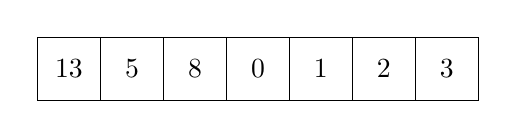
\begin{tikzpicture}
      \matrix (A) [matrix of nodes, nodes={draw, minimum size=8mm},
          column sep=-\pgflinewidth]{
          13 & 5 & 8 & 0 & 1 & 2 & 3\\};
    \end{tikzpicture}
  \end{center}
  \caption{A max heap and its array representation.}
\end{figure}

Heapsort, as you may imagine, utilizes a heap to sort elements. Heapsort
sorts its elements in two steps. The first step is involves creating the
heap. This means taking an array, and \emph{fixing} it such that it
obeys the constraints of a max or min heap. For our purposes, the heap
will be a max heap. The second step entails repeatedly ``removing'' the
largest element in the heap and ``placing'' it into the end of the
sorted array. This means that the root (the first element of the array)
is always the smallest element. Since Heapsort is an in-place algorithm,
we cannot simply remove an element from the heap and place it into the
sorted array; the heap and the sorted array are the same container. What
we can do is indicate where the end of the heap is, which also indicates
where each successive largest element should go. Each time the largest
element is selected, the heap has to be fixed. In the following Python
code for Heapsort, you will notice a lot of indices are shifted down by
1. Why is this? Recall how indices of children are computed. The formula
of the left child of $k$ being $2k$ only works assuming 1-based
indexing. We, in Computer Science, use 0-based indexing. So, we will run
the algorithm assuming 1-based indexing for the Heapsort algorithm
itself, subtracting 1 on each array index access to account for 0-based
indexing.

\begin{pythonlisting}{Heap maintenance in Python}
def max_child(arr, first, last):
    left = 2 * first
    right = left + 1
    if right <= last and arr[right - 1] > arr[left - 1]:
        return right
    return left

def fix_heap(arr, first, last):
    found = False
    parent = first
    great = max_child(arr, parent, last)

    while parent <= last // 2 and not found:
        if arr[parent - 1] < arr[great - 1]:
            arr[parent - 1], arr[great - 1] = arr[great - 1], arr[parent - 1]
            parent = great
            great = max_child(arr, parent, last)
        else:
            found = True
\end{pythonlisting}

\begin{pythonlisting}{Heapsort in Python}
def build_heap(arr, first, last):
    for parent in range(last // 2, first - 1, -1):
        fix_heap(arr, parent, last)

def heap_sort(arr):
    first = 1
    last = len(arr)
    build_heap(arr, first, last)
    for leaf in range(last, first, -1):
        arr[first - 1], arr[leaf - 1] = arr[leaf - 1], arr[first - 1]
        fix_heap(arr, first, leaf - 1)
\end{pythonlisting}


\section{Your Task}

\epigraph{\emph{Die Narrheit hat ein gro\ss{}es Zelt; Es lagert bei ihr alle
Welt, Zumal wer Macht hat und viel Geld.}}{---Sebastian Brant, \emph{Das
Narrenschiff}}

For this assignment you have 3 tasks:
\begin{enumerate}
  \item Implement Bubble Sort, Shell Sort, Quicksort, and Heapsort using
    the provided Python pseudocode in \textbf{C}. The interface for
    these sorts will be given as the header files \texttt{bubble.h},
    \texttt{shell.h}, \texttt{quick.h}, and \texttt{heap.h}.
    \textcolor{red}{You are not allowed to modify these files.}
  \item Implement a test harness for your implemented sorting
    algorithms. In your test harness, you will creating an array of
    random elements and testing each of the sorts. Your test harness
    \emph{must} be in the file \texttt{sorting.c}.
  \item Gather statistics about each sort and its performance. The
    statistics you will gather are the \emph{size} of the array, the
    number of \emph{moves} required, and the number of
    \emph{comparisons} required. \textcolor{red}{Note: a comparison is
    counted only when two array elements are compared.}
\end{enumerate}


\section{Specifics}

\epigraph{\emph{Vielleicht sind alle Drachen unseres Lebens
  Prinzessinnen, die nur darauf warten uns einmal sch\"on und mutig zu
sehen. Vielleicht ist alles Schreckliche im Grunde das Hilflose, das von
uns Hilfe will.}}{---Rainer Maria Rilke}

The following subsections cover the requirements of your test harness.
It is crucial that you follow the instructions.

\subsection{Command-line Options}

Your test harness must support any combination of the following
command-line options:

\begin{itemize}
  \item \texttt{-a}\ : Employs \emph{all} sorting algorithms.
  \item \texttt{-b}\ : Enables Bubble Sort.
  \item \texttt{-s}\ : Enables Shell Sort.
  \item \texttt{-q}\ : Enables Quicksort.
  \item \texttt{-h}\ : Enables Heapsort.
  \item \texttt{-r seed}\ : Set the random seed to \texttt{seed}.
    The \emph{default} seed should be 7092016.
  \item \texttt{-n size}\ : Set the array size to \texttt{size}. The
    \emph{default} size should be 100.
  \item \texttt{-p elements}\ : Print out \texttt{elements} number of
    elements from the array. The \emph{default} number of elements to
    print out should be 100. \textcolor{red}{If the size of the array is
      less than the specified number of elements to print, print out the
    entire array and nothing more.}
\end{itemize}

It is important to read this \emph{carefully}. None of these options are
\emph{exclusive} of any other (you may specify any number of them,
including \emph{zero}). The most natural data structure for this
problem is a \emph{set}.

\subsection{Sets}

For this assignment, you are required to implement simple
\emph{sets} using bits to track which command-line options are specified
when your program is run. The number of bits will be small, but in
subsequent assignments you will be implementing sets for an
\emph{arbitrary} number of bits. Your set will be initialized using an
unsigned int of a size equivalent to the number of bits as shown below.

\begin{codelisting}{}
typedef uint32_t Set;
\end{codelisting}

For manipulating the bits in a set, we use bit-wise operators. These
operators as the name suggests will perform an operation on every bit in
a number. The following are the six bit-wise operators specified in
\textbf{C}:

\begin{center}
  \begin{tabular}{|c|l|l|}
    \hline
    \verb|&| & bit-wise AND & Performs the AND operation on every bit
    of two numbers. \\
    \hline
    \verb||| & bit-wise OR & Performs the OR operation on every bit of
    two numbers. \\
    \hline
    \verb|~| & bit-wise NOT & Inverts all bits in the given number. \\
    \hline
    \verb|^| & bit-wise XOR & Performs the exclusive-OR operation on
    every bit of two numbers. \\
    \hline
    \verb|<<| & left shift & Shifts bits in a number to the left by a
    specified number of bits. \\
    \hline
    \verb|>>| & right shift & Shifts bits in a number to the right by a
    specified number of bits. \\
    \hline
  \end{tabular}
\end{center}

\noindent Recall that the basic set operations are: \emph{membership},
\emph{union}, \emph{intersection} and \emph{negation}. For this
assignment you will be implementing functions for these operations and a
few more helper functions. Using these functions, you will set (make the
bit 1) or clear (make the bit 0) bits in the \texttt{Set} depending on
the command-line options read by \texttt{getopt()}. You can then check
the states of all the bits (the members) of the \texttt{Set} using a
single \texttt{for} loop and execute the corresponding sort. Note: you
will not use all of the functions, but we will check their presence in
\texttt{set.c}. Again, you \emph{must} use sets to track which
command-line options are specified when running your program.

\subsubsection{\texttt{Set set\_empty(void)}}

This function is used to return an empty set. In this context, an empty
set would be a set in which all bits are equal to 0.

\subsubsection{\texttt{bool set\_member(Set s, uint8\_t x)}}

\begin{align*}
  x \in s \iff x\, \text{is a member of set}\, s
\end{align*}

% return (1 << x) & A
\noindent This function returns a \texttt{bool} indicating the presence
of the given value \texttt{x} in the set \texttt{s}. You will use the
bit-wise AND operator to determine set membership. The first operand for
the AND operation is the set \texttt{s}. The second operand is the value
obtained by left shifting 1 \texttt{x} number of times. If the result of
the AND operation is a non-zero value, then \texttt{x} is a member of
\texttt{s} and \texttt{true} is returned to indicate this. Return
\texttt{false} if the result of the AND operation is 0.

\subsubsection{\texttt{Set set\_insert(Set s, uint8\_t x)}}

This function returns a set with the bit corresponding to \texttt{x}
equal to 1. Here, the bit is set using the bit-wise OR operator. The
first operand for the OR operation is the set \texttt{s}. The second
operand is value obtained by left shifting 1 by \texttt{x} number of
bits.

\subsubsection{\texttt{Set set\_remove(Set s, uint8\_t x)}}

Similar to insertion, removing a member from the set means to clear the
bit corresponding to \texttt{x}. Here, the bit is cleared using the
bit-wise AND operator. The first operand for the AND operation is the
set \texttt{s}. The second operand is a negation of the number 1 left
shifted to the same position that \texttt{x} would occupy in the set.
This means that the second operand would be all 1s except for the bit at
\texttt{x}'s position. The function returns set \texttt{s} after
removing \texttt{x}.

\subsubsection{\texttt{Set set\_intersect(Set s, Set t)}}

\begin{align*}
  s \cap t = \{x | x \in s \land x \in  t\}
\end{align*}

% return A & B
An intersection of two sets is a collection of elements that are common
to both sets. Here, to calculate the intersection of the two sets,
\texttt{s} and \texttt{t} we need to use the AND operator. Only the bits
corresponding to members in both \texttt{s} and \texttt{t} need to be
equal to 1 and the new set is returned by the function.

\subsubsection{\texttt{Set set\_union(Set s, Set t)}}

\begin{align*}
  s \cup t = \{x | x \in s \lor x \in  t\}
\end{align*}

% return A | B
A union of two sets is a collection of all elements in both sets. Here,
to calculate the union of the two sets, \texttt{s} and \texttt{t} we
need to use the OR operator. The bits corresponding to members in
\texttt{s} or \texttt{t} equal to 1 therefore are in the new set is
returned by the function.

\subsubsection{\texttt{Set set\_complement(Set s)}}

This function is used to return the complement of a given set. By
complement we mean that all bits in the set are flipped using the NOT
operator.

\subsubsection{\texttt{Set set\_difference(Set s, Set t)}}

The difference of two sets refers to the elements of set \texttt{s}
which are not in set \texttt{t}. In other words, it refers to the
members of set \texttt{s} that are unique to set \texttt{s}. The
difference is calculated using the AND operator where the two operands
are set \texttt{s} and the negation of set \texttt{t}.

This function can be used to find the complement of a given set as well,
in which case the first operand would be the universal set $\mathbb{U}$
and the second operand would be the set you want to complement as shown
below.

\begin{align*}
  \overline{s} = \{ x | x \notin s\} = \mathbb{U} -s
\end{align*}

\subsection{Testing}

\begin{itemize}
  \item You will test each of the sorts specified by command-line option
    by sorting an array of pseudorandom numbers generated with
    \texttt{random()}. Each of your sorts should sort the \emph{same}
    pseudorandom array. \textcolor{red}{Hint: make use of
    \texttt{srandom()}.}
  \item The pseudorandom numbers generated by \texttt{random()} should
    be \emph{bit-masked} to fit in \emph{30} bits. \textcolor{red}{Hint: use
    bit-wise AND.}
  \item Your test harness \emph{must} be able to test your sorts with
    array sizes \emph{up to the memory limit of the computer}. That
    means that you will need to dynamically allocate the array.
  \item Your program should have no \emph{memory leaks}. Make sure you
    \texttt{free()} before exiting. \texttt{valgrind} should pass
    cleanly with any combination of the specified command-line options.
  \item Your algorithms \emph{must} correctly sort. Any algorithm that
    does not sort correctly will receive a \emph{zero}.
\end{itemize}

A large part of this assignment is understanding and comparing the
performance of various sorting algorithms. You essentially conducting an
experiment. As stated in \S 6, you \emph{must} collect the following
statistics on each algorithm:

\begin{itemize}
  \item The \emph{size} of the array,
  \item The number of \emph{moves} required (each time you transfer an
    element in the array, that counts), and
  \item The number of \emph{comparisons} required (comparisons
    \emph{only} count for \emph{elements}, not for logic).
\end{itemize}

\subsection{Output}

The output your test harness produces \emph{must} be formatted like in
the following examples:

\begin{lstlisting}[style=bashstyle]
  $ ./sorting -bq -n 1000 -p 0
  Bubble Sort
  1000 elements, 733833 moves, 498972 compares
  Quick Sort
  1000 elements, 6975 moves, 14190 compares
  $ ./sorting -bq -n 15 -r 2021
  Bubble Sort
  15 elements, 228 moves, 105 compares
       45003895     46620555    199644728    203770850    218081181
      230022357    273593510    314322227    377988577    458735007
      553822818    570456718    653251166    802708864    890975627
  Quick Sort
  15 elements, 60 moves, 98 compares
       45003895     46620555    199644728    203770850    218081181
      230022357    273593510    314322227    377988577    458735007
      553822818    570456718    653251166    802708864    890975627
\end{lstlisting}

For each sort that was specified, print its name, the statistics for the
run, then the specified number of array elements to print. The array
elements should be printed out in a table with 5 columns. Each array
element should be printed using the following \texttt{printf()}
statement:

\begin{codelisting}{}
printf("%13" PRIu32); // Include <inttypes.h> for PRIu32.
\end{codelisting}

\medskip
\begin{prelab}{Pre-lab Part 4}
    \begin{enumerate}
        \item Explain how you plan on keeping track of the number of
          moves and comparisons since each sort will reside within its
          own file.
    \end{enumerate}
\end{prelab}


\section{Deliverables}

\epigraph{\emph{Dr.\ Long, put down the Rilke and step away from the
computer.}}{---Michael Olson}

You will need to turn in:

\begin{enumerate}
  \item Your program \emph{must} have the following source and header files:
  \begin{itemize}
    \item Each sorting method will have its own pair of header file and source file.
    \begin{itemize}
      \item \texttt{bubble.h} specifies the interface to \texttt{bubble.c}.
      \item \texttt{bubble.c} implements Bubble Sort.
      \item \texttt{gaps.h} contains the Pratt gap sequence for Shell
        Sort.
      \item \texttt{shell.h} specifies the interface to \texttt{shell.c}.
      \item \texttt{shell.c} implements Shell Sort.
      \item \texttt{quick.h} specifies the interface to \texttt{quick.c}.
      \item \texttt{quick.c} implements Quicksort.
      \item \texttt{stack.h} specifies the interface to the stack ADT.
      \item \texttt{stack.c} implements the stack ADT.
      \item \texttt{heap.h} specifies the interface to \texttt{heap.c}.
      \item \texttt{heap.c} implements Heap Sort.
      \item \texttt{set.h} specifies the interface to the set ADT.
      \item \texttt{set.c} implements the set ADT.
    \end{itemize}
    \item \texttt{sorting.c} contains \texttt{main()} and \emph{may}
      contain any other functions necessary to complete the assignment.
  \end{itemize}

You can have other source and header files, but \emph{do not try to be
overly clever}. The header files for each of the sorts are provided to
you. Each sort function takes the array of \texttt{uint32\_t}s to sort
as the first parameter and the length of the array as the second
parameter.

  \item \texttt{Makefile}: This is a file that will allow the grader to
    type \texttt{make} to compile your program. Typing \texttt{make}
    must build your program and \texttt{./sorting} alone as well as
    flags must run your program.

    \begin{itemize}
      \item \texttt{CFLAGS=-Wall -Wextra -Werror -Wpedantic}
        must be included.
      \item \texttt{CC=clang} must be specified.
      \item \texttt{make clean} must remove all files that are compiler
        generated.
      \item \texttt{make} should build your program, as should
        \texttt{make all}.
      \item Your program executable \emph{must} be named
        \texttt{sorting}.
    \end{itemize}

  \item Your code must pass \texttt{scan-build} \emph{cleanly}.

  \item \texttt{README.md}: This \emph{must} be in \emph{markdown}.
    This must describe how to use your program and \texttt{Makefile}.

  \item \texttt{DESIGN.pdf}: This \emph{must} be a PDF. The design
    document should contain answers to the pre-lab questions at the
    beginning and describe your design for your program with enough
    detail that a sufficiently knowledgeable programmer would be able to
    replicate your implementation.  This does not mean copying your
    entire program in verbatim. You should instead describe how your
    program works with supporting pseudo-code.  \textcolor{red}{You
      \emph{must} push the \texttt{DESIGN.pdf} before you push
    \emph{any} code.}

  \item \texttt{WRITEUP.pdf}: This document \emph{must} be a PDF. The
    writeup must include the following:
    \begin{itemize}
      \item Identify the respective time complexity for each sort and
        include what you have to say about the constant.
      \item What you learned from the different sorting algorithms.
      \item How you experimented with the sorts.
      \item Graphs explaining the performance of the sorts on a variety
        of inputs, such as arrays in reverse order, arrays with a small
        number of elements, and arrays with a large number of elements.
      \item Analysis of the graphs you produce.
    \end{itemize}
\end{enumerate}


\section{Submission}

\epigraph{\emph{Da\ss{} Gott ohn Arbeit Lohn verspricht, Verla\ss{} dich
darauf und backe nicht Und wart, bis dir 'ne Taube gebraten Vom Himmel
k\"onnt in den Mund geraten!}}{---Sebastian Brant, \emph{Das
Narrenschiff}}

To submit your assignment, refer back to \texttt{assignment0} for the
steps on how to submit your assignment through \texttt{git}.  Remember:
\emph{add, commit,} and \emph{push}!

\textcolor{red}{Your assignment is turned in \emph{only} after you have
  pushed \emph{and} submitted the commit ID on Canvas. If you forget to
  push, you have not turned in your assignment and you will get a
  \emph{zero}. ``I forgot to push'' is not a valid excuse. It is
\emph{highly} recommended to commit and push your changes \emph{often}.}


\section{Supplemental Readings}

\epigraph{\emph{The more you read, the more things you will know. The more that
you learn, the more places you'll go.}}{---Dr.\ Seuss}\noindent

\begin{itemize}
    \item \textit{The C Programming Language} by Kernighan \& Ritchie
    \begin{itemize}
	\item Chapter 1 \S 1.10
	\item Chapter 3 \S 3.5
        \item Chapter 4 \S 4.10--4.11
        \item Chapter 5 \S 5.1--5.3 \& 5.10
    \end{itemize}
     \item  \emph{C in a Nutshell} by T.\ Crawford \& P.\ Prinz.
     \begin{itemize}
      \item Chapter 6 -- Example 6.5		% Not a section
      \item Chapter 7 -- Recursive Functions
      \item Chapter 8 -- Arrays as Arguments of Functions
      \item Chapter 9 -- Pointers to Arrays
      \end{itemize}
\end{itemize}
\centerline{
\includegraphics[height=2in]{monkey.jpeg}}
\end{document}
